\documentclass[10pt]{article}
\usepackage[margin=0.8in]{geometry}
\usepackage[T1]{fontenc}
\usepackage[utf8]{inputenc}
\usepackage{lmodern,microtype}
\usepackage{graphicx,booktabs,multicol}
\usepackage{amsmath}
\usepackage[hidelinks]{hyperref}
\usepackage{caption}
\captionsetup{font=footnotesize,labelfont=bf,skip=3pt}
\setlength{\parskip}{2pt}
\setlength{\parindent}{0pt}
\usepackage{titlesec}
\titlespacing*{\section}{0pt}{7pt}{2pt}
\titleformat{\section}{\normalsize\bfseries}{\thesection.}{0.5em}{}
\usepackage{enumitem}
\setlist{nosep,leftmargin=1.2em}

\title{\vspace{-22pt}\large\textbf{13F Positioning Factors --- Memo}}
\author{\normalsize Lucas Silva}
\date{\normalsize August 2026}

\begin{document}
\maketitle
\vspace{-26pt}

{\footnotesize\emph{Compressed from the full technical report
(\texttt{docs/paper/main.pdf}, 30 pp.), which carries every
construction, pre-registration, surface, negative result, and one
explicit retraction. Reproduction: \texttt{python bootstrap.py \&\&
python run\_experiments.py} from a clean clone (EDGAR needs only a
contact e-mail; prices auto-fetch).}}

\section{Factor hypothesis}

13F filings are stale (up to 45 days), long-only, quarterly: most of
their content is already in prices. Our premise: a premium can only
live where the filing reveals an action that was \emph{costly to
take} or \emph{impossible to avoid}; ownership \emph{states} ---
crowding, concentration, breadth, days-of-ADV, factor tilt --- carry
no direction. The premise was stress-tested against a six-class
taxonomy (17 catalogue signals with literature anchors, 5
pre-registered interactions, 9 smart-money designs, 15 crowding
formulations, latent-structure and event-clock studies; $\sim$60
experiments, every one with its pre-registration in the script
docstring) and survived as two factors and two empirical laws.
\textbf{Law 1: states have no arrow} (15 crowding formulations dead
at every clock --- graph diffusion, centrality, absorption,
strategy-crowding included; states earned only two jobs:
denominators and risk conditioning). \textbf{Law 2: distress is
information when observed, never predicted} (contemporaneous forced
selling $t\approx+10$; every anticipation design --- daily synthetic
stress, quarterly Coval--Stafford-style flow forecasts (OOS rank-corr
$-0.015$), crash cascades --- failed its mechanism gate or died on
the full panel).

\textbf{NCB --- New-Conviction Breadth} (long). Per stock, the share
of filers opening or growing ($\ge$1.25$\times$, split-adjusted by a
holder-consensus modal-ratio detector, validated 6/6) a position in
the \emph{top decile of their own book}; residualized on
$\log$mktcap$+\log$ADV because a formal placebo (dart-throwing
value-weighted managers) shows the raw count is mechanically
size-loaded. Mechanism: top-of-book room is made by displacing
existing conviction --- expensive, deliberate, and impossible to
produce by indexing or inflows; counting it across independent
managers aggregates only paid-for opinion. Results: $+1.9\%$/q
spread, $t=+3.44$, Sharpe $\approx$1.0, IC $+0.023$ (fundamental
law: $0.023\times\sqrt{1900}\approx1.0$ --- breadth, not per-name
accuracy). Only entry clearing the catalogue-wide Bonferroni bar
($t\ge3.2$, 34 tests); 8 implementation replications in a
$t=3.3$--$4.0$ band across two data vintages; survives random 50\%
coverage halvings ($t=+3.45/+2.79$); joint Fama--MacBeth premium
$t=+3.04$ holding six classical characteristics and three other 13F
signals simultaneously; unabsorbed by IPCA latent factors
(spanning $t\approx+6$). Hyperparameters (0.90 weight-quantile /
1.25 growth / 5 min holders) fixed a priori, never tuned; the full
$4{\times}3{\times}3$ surface, mapped later under a coupled
block-bootstrap 5th-percentile protocol (arXiv:2510.12725), is
\emph{uniformly positive} out-of-sample (all 36 configs OOS Sharpe
$+1.05$ to $+2.53$; in-sample ranks OOS at $+0.53$, so selection is
meaningful; the a-priori default sits mid-surface, conservative).

\textbf{FSS --- Forced-Sale Supply} (short). Implied flow
$=\mathrm{AUM}_t/\mathrm{AUM}_{t-1}-(1+r^{\mathrm{book}})$ separates
client/leverage money from market growth. Validated on behavior, not
returns: flow$<-10\%$ managers sell \textbf{34.5\%} of remaining
shares the \emph{following} quarter vs 23.1\% for healthy
($t\approx+10$ at every cut from $-5\%$ to $-20\%$ --- monotone
curve, not a fitted number; selling is $\approx$pro-rata across
liquidity, correlation $-0.02$). Stock supply
$=\sum_{\mathrm{dis}}|\mathrm{flow}|{\cdot}\mathrm{AUM}{\cdot}w/
\mathrm{ADV}$. Price: index-hedged, all 15 threshold$\times$basket
configs are flat 2013--20 (Sharpe $-0.1$ to $-0.5$) and pay 2021--25
($+0.6$ to $+1.0$, $t$ to $+4.0$) --- a \emph{regime}
(degrossing/rates), not a hyperparameter: IS-to-OOS rank correlation
across configs is $-0.81$, so in-sample selection is refused and the
a-priori spec ships. Benchmark honesty: an early
``$-4.5\%$/q vs universe mean'' figure was skewness (the
cross-sectional mean sits $\sim$4\%/q above the median); the hedged
number is the true one. The pressure autopsy explains why generic
flow-pressure fails (impact realized inside the filing quarter;
orthogonalized to momentum/reversal nothing remains) and why FSS
works: liquidation \emph{continues} past disclosure only when
selling is forced --- condition on the agent's constraint, not the
asset's state. The pre-registered pressure$\times$vol interaction
(E4) died properly: smoke$\to t{=}+2.06$ old universe $\to+0.77$ on
complete books; its identification autopsy (vol vs ADV vs mktcap)
had already returned ``no formal claim.''

\section{Scope decisions and deliberate exclusions}

\textbf{2013Q2--2025Q4}: the window where two independent ingestion
paths (DERA structured datasets; raw EDGAR parsing) overlap and
cross-validate (row counts and value totals per sampled filing;
$<$95\% agreement halts the pipeline). \textbf{Universe: the full
filer census} (2{,}793$\to$7{,}693) --- a measured choice, not a
default: activity/concentration/patience/performance filters hurt
(up to $t=-3.25$) or do nothing; the passive question closed on
three fronts (index complexes $=$ 1/3 of AUM, 1\% of conviction
votes, removal moves the spread 6 bps; ETF purge inside books
changes vote-sets of 25\% of managers yet leaves the ranking at
correlation 0.974 --- uniform contamination is innocuous, unlike
splits, which are differential and required the detector).
\textbf{Assets}: common equities, mapped current ticker, \$1 floor;
options excluded (no deltas), ETF instruments excluded (never in the
price panel --- 1 of 7{,}886 audited ETF ids maps). \textbf{Not
pursued, with evidence}: smart-money weighting (0-of-9; skill
persistence 0.25 and $\perp$ holdings --- reweighting the electorate
is reweighting at random); imitation of books (the median \$1B+
filer loses $-3.3\%$/yr to the S\&P before fees, 13\% positive-IR:
Bessembinder composition arithmetic --- the alpha is in flows
\emph{between} managers, not in the books); window dressing (both
pre-registered signs wrong; placebo follows thesis; a Q4-only
reversal of $-1.9\%$ is an 11-observation footnote);
amendment-following (materials price \emph{against} the correction,
$t=-3.5$); daily stress anticipation (\textbf{retracted}, below).

\section{Data engineering and point-in-time discipline}

\textbf{Bitemporal store}: every row carries period and EDGAR
acceptance timestamp; research reads holdings only through
\texttt{as\_of(period, knowledge\_date)}, materializing current and
prior quarter at the same vantage --- late filings, amendments, and
restatements cannot leak. Amendment semantics from cover pages
(restatement replaces; NEW HOLDINGS --- lapsed confidential
treatment --- adds; missing $=$ conservative restatement; an
amendment is a version, never a competing filing). Value scale
detected per filing (the 2022--23 thousands/dollars cutover keys on
filing date). Identity: union-find on explicit evidence; name
similarity only proposes; merges need a human entry. \textbf{The
D+45 clock is measured, not assumed}: across 254{,}630 filings,
median delay 41 days, 49.9\% by D+40, 89.4\% by D+45, 98.1\% by
D+60, p99 $=$ 128d; lateness is sticky (41\% repeat); per-name
ragged entry adds $+0.2\%$/yr ($t\approx0$) over the batch clock.
Forward returns start the first trading day \emph{after} decision.
\textbf{The crosswalk is a result}:
CUSIP$\to$issuer-name$\to$current ticker; renames correct by
construction, recycling fails closed (4.5\% flagged), CUSIP
reassignment measured at 0.22\% of exit flow. A value-weighted audit
found \textbf{46.4\% of book value unmapped} (EDGAR abbreviations
defeat exact matching precisely on mega-caps; count-weighted
coverage had looked fine --- audits must be value-weighted). Fix:
top-250 CUSIPs hand-verified (63$\to$85.4\% of non-ETF value), then
a \textbf{24-run re-verification campaign}: 21 verdicts stable; two
instruments \emph{strengthened} (flow contrast $t=13.8\to20.9$;
synthetic short interest vs real, corr $0.47\to0.55$); one result
\textbf{retracted} --- a daily stress-anticipation short
($t=-2.16\to+0.37$ on complete books; an eligibility-selection
artifact the funnel had already declined to promote).
\textbf{Survivorship measured}: the price panel conditions on
survival to download (nothing dies inside a window --- verified);
the unmapped tail is 33\% of eligible-instrument value with an NCB
vote rate only $+0.002$ different ($t=+2.4$); the delisting
truncations (bankruptcies missing from the no-vote quintile,
takeover premia from conviction names) both cut \emph{against} the
measured spread. CRSP closes both (85.4$\to\sim$98\%).

\begin{table}[h]
\centering\scriptsize
\caption{The re-verification campaign in brief (full table in the
report): pre-registered expectation was levels move where mega-caps
matter, verdicts stand.}
\begin{tabular}{lccl}
\toprule
result & old universe & expanded & verdict \\
\midrule
NCB (residualized) & $t=+3.67/+3.83/+3.27$ & $t=+3.44$ & in band; 8th replication \\
flow instrument & $t=+13.8$ & $t=+20.9$ & \textbf{stronger} with complete books \\
synthetic short interest & corr $+0.47$ & $+0.55$ & \textbf{stronger} \\
FM joint $\lambda$ (NCB / dbreadth) & $+3.26/+4.62$ & $+3.04/+4.01$ & holds \\
pressure$\times$vol flicker & $t=+2.06$ & $+0.77$ & died on fuller data \\
median fund excess & $-5.0\%$/yr & $-3.3\%$/yr & level moved as predicted \\
daily stress-anticipation & $t=-2.16$ & $t=+0.37$ & \textbf{retracted} (artifact) \\
\bottomrule
\end{tabular}
\end{table}

\section{Evaluation protocol and backtest methodology}

One protocol, fixed ex-ante: quintile portfolios, Q5$-$Q1 on forward
quarterly returns (sums of daily simple returns ---
quintile-neutral convention), Newey--West $t$ (4 lags on
non-overlapping series $=$ conservative), Spearman IC, seeded random
tie-breaks (alphabetical ties fabricate signal at mass points).
\textbf{Why the EW base}: the evaluation question is ``does the
ranking order returns?'', under which every name is one observation
--- value-weighting collapses effective $N$ onto a handful of
mega-caps and breaks the $\mathrm{IC}\sqrt{N}$ arithmetic the
signals live on; EW is the \emph{measurement} convention,
cap-weighting the \emph{implementation} convention (engine and LO
below), VW reported as the bridge (indicative: its weight panel's
corrupt tail is documented). \textbf{Why residualize}: a formal
placebo --- dart-throwing value-weighted managers --- decides
neutralization per signal, ex ante: if uninformed books produce the
size/liquidity correlation mechanically, the headline is the
cross-sectional residual on $\log$mktcap$+\log$ADV; otherwise raw.
One rule, two opposite unmaskings: NCB raw is \emph{nothing}
($t=-0.9$; the mechanical large-cap drag masks the information ---
the residual is where the signal lives, $t=+3.5$), while days-of-ADV
raw replicates its published point and dies residualized ($t=-0.4$)
--- the published crowding effect \emph{was} size/liquidity.
Verdicts are paired quarter-by-quarter deltas on common samples;
families carry Bonferroni bars with iteration counts; post-hoc
entrants are candidates, never promotions; smoke never decides (four
smoke mirages died on full panels). \textbf{Engine}: tradable universe
(\$4/\$5M ADV/252d), 20\% tails, 40-name leg minimum, rebalance at
each signal's decision dates, \textbf{5 bps/side} (in line with
realized institutional costs; quarterly trading, measured one-way
turnover 3--7$\times$/yr, and the tradability filter is the
liquidity control keeping slippage second-order; impact belongs to
capacity, not backtests), \textbf{50 bps borrow} (at 200 bps
hard-to-borrow the FSS leg loses $\approx$1.5\%/yr, Sharpe
0.85$\to$0.73 --- survives). Combo legs weighted \emph{equally by
design} (no-optimization default).

\section{Results}

\begin{table}[h]
\centering\scriptsize
\caption{Net production results (5 bps/side; 50 bps borrow;
expanded universe). Cost $=$ measured commission drag (net minus
zero-fee run); turn $=$ implied one-way annual turnover. LO rows:
excess/TE/IR vs own benchmark; the cap-weighted 500 proxy tracks
the actual S\&P at 2.7\% TE ($-0.6\%$/yr drift).}
\begin{tabular}{lrrrrrr}
\toprule
strategy & ann.\ net & vol & Sharpe & maxDD & cost (bps/y) & turn \\
\midrule
\textbf{NCB$+$FSS book} & $+6.2\%$ & $6.0\%$ & $\mathbf{+1.02}$ & $-10.6\%$ & 67 & 6.7$\times$ \\
FSS short leg & $+10.4\%$ & $12.2\%$ & $+0.85$ & $-26.1\%$ & 65 & 6.5$\times$ \\
NCB (residualized) & $+2.9\%$ & $6.7\%$ & $+0.42$ & $-18.7\%$ & 65 & 6.5$\times$ \\
FM score (10 predictors) & $+4.0\%$ & $16.9\%$ & $+0.24$ & $-62.1\%$ & 43 & 4.3$\times$ \\
\bottomrule
\end{tabular}
\end{table}
\vspace{-4pt}

\textbf{Long-only expression.} A naive EW long basket against the
S\&P is condemned by the composition arithmetic above (the
Bessembinder tax the median 13F book itself pays); the institutional
design tilts a genuine cap-weighted model --- top-500 by repaired
market cap, validated at 2.7\% TE to the actual index --- by the
combo rank, MSCI-style multiplicative exponential (positivity
preserved, unscored names stay at benchmark weight). IR
$\approx$0.5--0.6, roughly \emph{flat in tilt strength}: the
signature of a scalable signal, with $k$ shipped as a tracking-error
budget (Table~\ref{tab:lo}, Figure~\ref{fig:lo}).

\begin{table}[h]
\centering\scriptsize
\caption{Long-only cap-weighted model and combo tilts, net of
5 bps/side, quarterly. Excess/TE/IR and relative maxDD (worst
peak-to-trough of the log wealth ratio) vs the tilt's own benchmark;
last row vs the actual S\&P.}
\label{tab:lo}
\begin{tabular}{lrrrrrrrr}
\toprule
portfolio & total net & vol & Sharpe & maxDD & excess & TE & IR & rel.\ DD \\
\midrule
S\&P 500 (actual index) & $+14.8\%$ & $17.1\%$ & $0.86$ & $-41\%$ & --- & --- & --- & --- \\
cap-weighted 500 (proxy) & $+14.1\%$ & $18.0\%$ & $0.78$ & $-45\%$ & --- & --- & --- & --- \\
combo tilt $k{=}0.5$ & $+14.6\%$ & $18.2\%$ & $0.80$ & $-45\%$ & $+0.4\%$ & $0.9\%$ & $0.49$ & $-2.5\%$ \\
combo tilt $k{=}1$ \textbf{(default)} & $+15.1\%$ & $18.4\%$ & $0.82$ & $-45\%$ & $+1.0\%$ & $1.8\%$ & $0.53$ & $-5.7\%$ \\
combo tilt $k{=}2$ & $+16.4\%$ & $19.2\%$ & $0.85$ & $-44\%$ & $+2.2\%$ & $4.0\%$ & $0.57$ & $-13.7\%$ \\
combo tilt $k{=}3$ & $+17.7\%$ & $20.4\%$ & $0.87$ & $-44\%$ & $+3.6\%$ & $6.2\%$ & $0.58$ & $-21.2\%$ \\
tilt $k{=}3$ vs S\&P (actual) & & & & & $+2.9\%$ & $7.3\%$ & $0.40$ & $-25.5\%$ \\
\bottomrule
\end{tabular}
\end{table}

\begin{figure}[h]
\centering
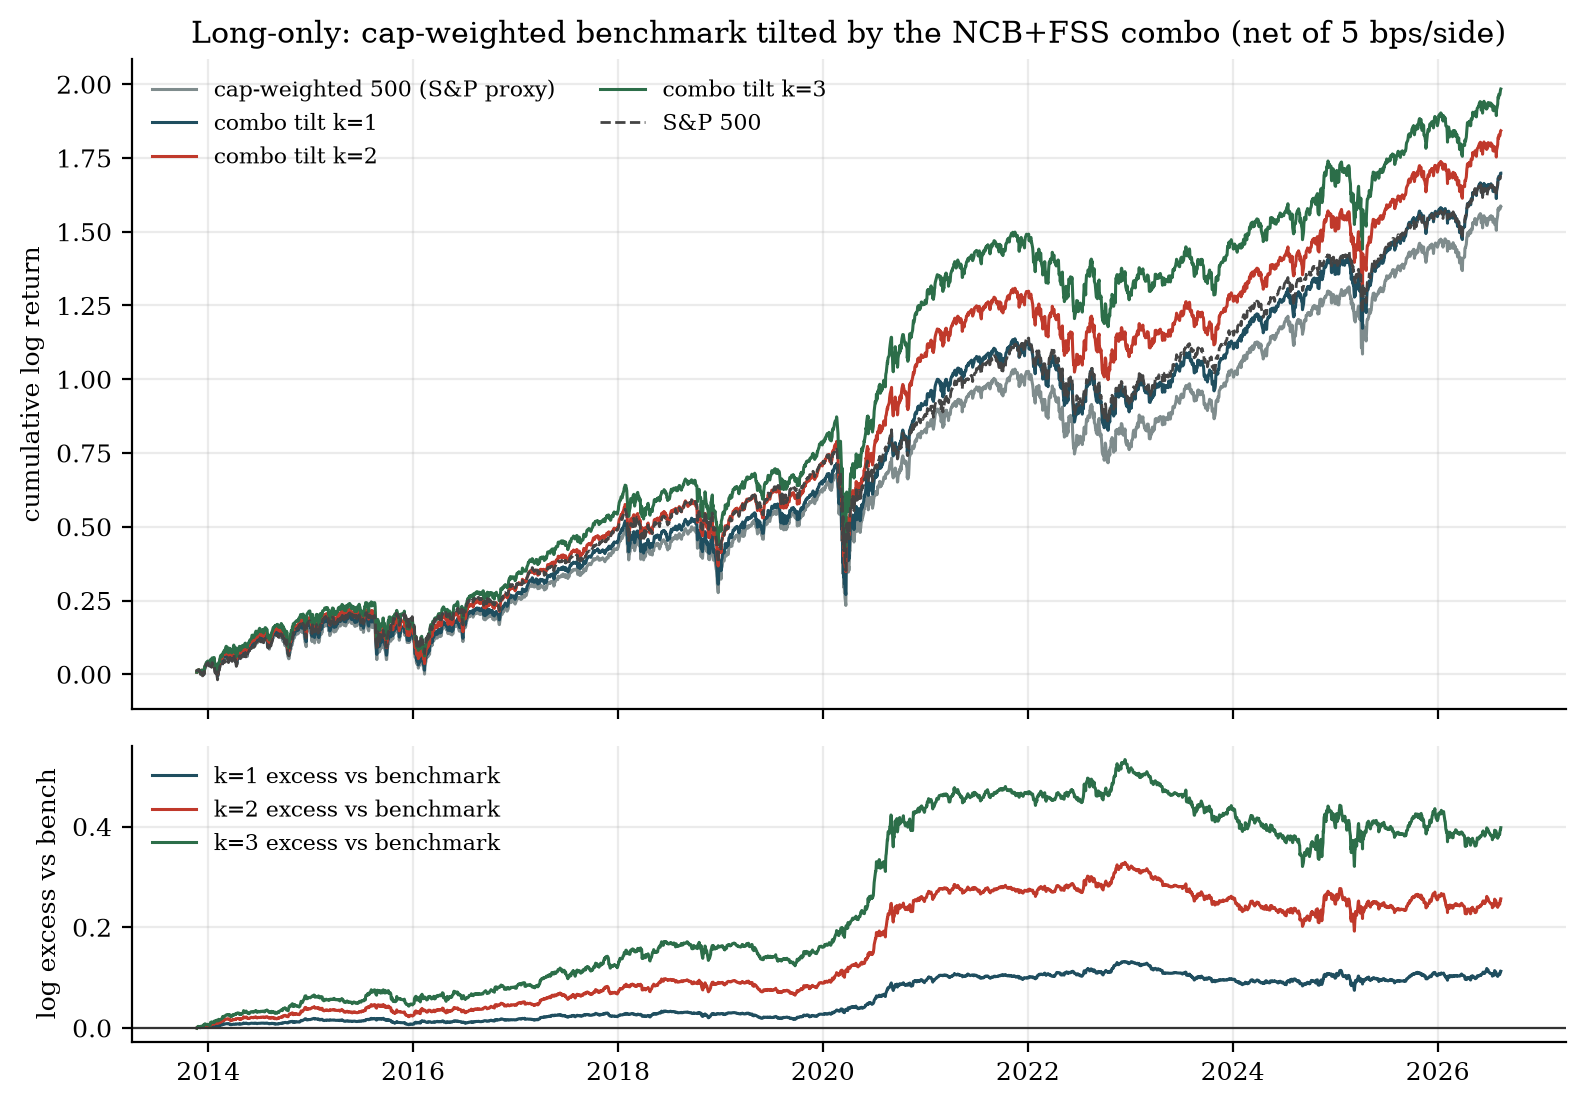
\includegraphics[width=.8\linewidth]{figs/f11_long_only.png}
\vspace{-6pt}
\caption{Long-only benchmark tilt, net (log cumulative). Top:
levels; bottom: log excess vs the benchmark by tilt strength.}
\label{fig:lo}
\end{figure}

\begin{figure}[h]
\centering
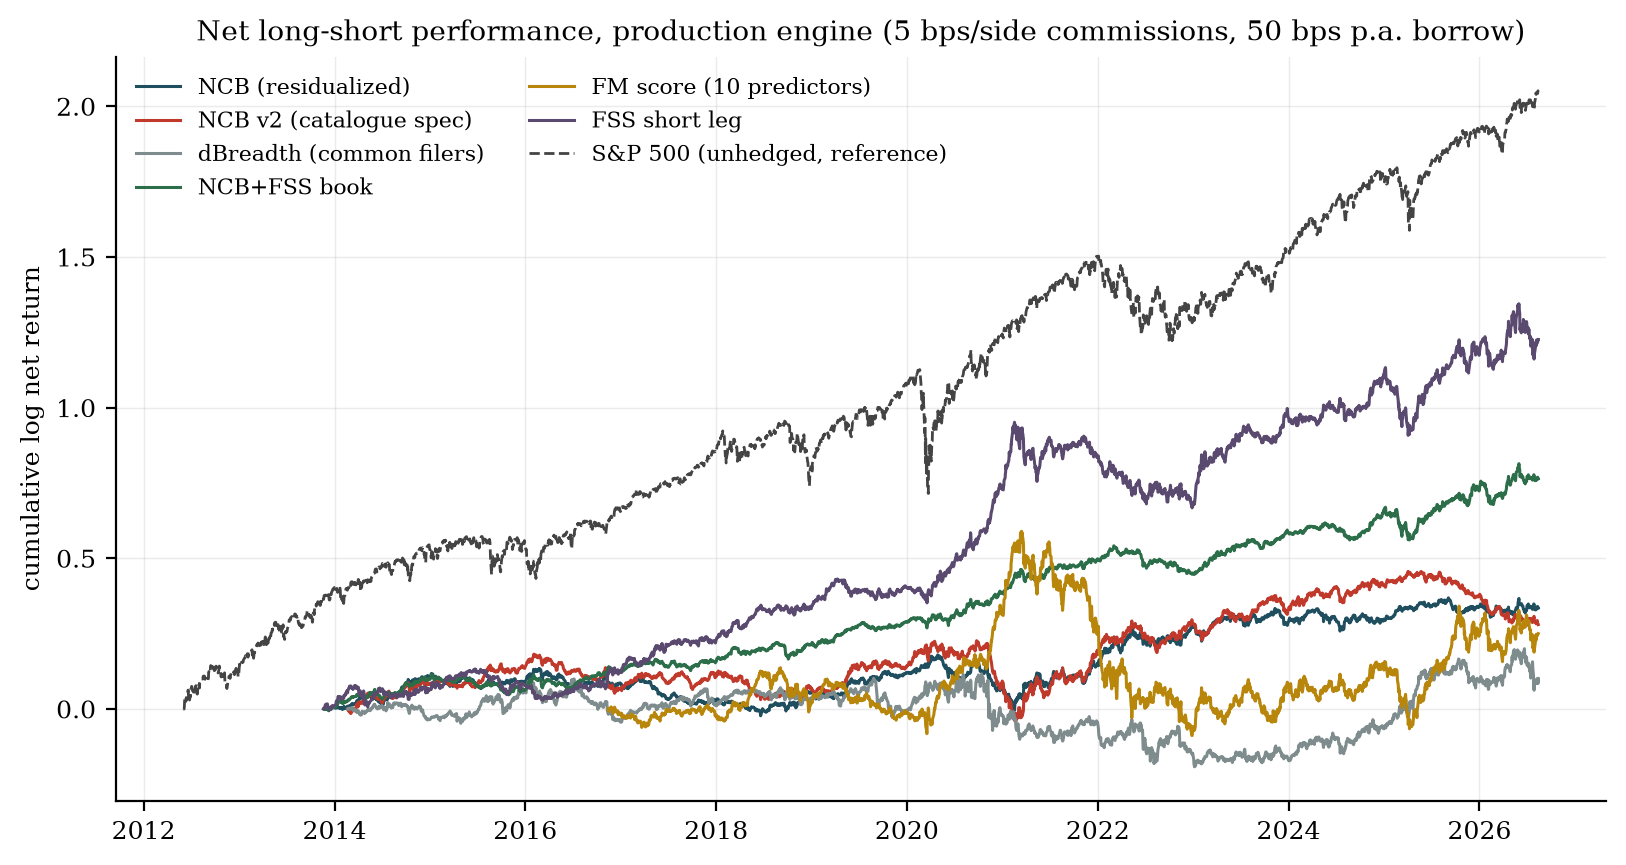
\includegraphics[width=.88\linewidth]{figs/f1_engine_curves.png}
\vspace{-6pt}
\caption{Net long-short performance, production engine (log
cumulative; 5 bps/side, 50 bps p.a.\ borrow, expanded universe).}
\end{figure}

\textbf{Combining models.} Three combiner schools raced strictly OOS
on ten pre-registered predictors: Fama--MacBeth/Lewellen wins the
research protocol (Sharpe 0.86 vs IC-weighted 0.69 and naive 0.74;
A$-$C paired $t=+1.96$); joint marginality: NCB $\lambda\,t=+3.04$,
breadth-change $t=+4.01$ (an \emph{ingredient}: weak solo, strong
jointly --- it also replicates Chen--Hong--Stein at $+1.65\%$/q).
The engine decomposition is a result: the FM book nets 0.24 with a
$-62\%$ drawdown because its two biggest premia (size $t=+4.45$,
liquidity $t=+4.39$) live outside the tradable set --- on the
tradable universe, residualized, the FM ranking retains
\emph{nothing} ($t=-0.70$); the tradable alpha is its 13F
components, hence the NCB$+$FSS book. IPCA (Kelly--Pruitt--Su,
verified against the authors' package): $W_\alpha$ cannot reject at
$T{=}50$ ($p=0.4$--$0.6$, power); unrestricted OOS Sharpe 0.97
beats FM paired ($t=+2.08$) but is a post-hoc entrant $\Rightarrow$
candidate, FM remains production; the spanning answer stands (no
latent factor absorbs NCB). An ML cross-check (ridge/kNN/boosting/RF
on the 12 change variables, walk-forward, market$+$size-residualized
rank target) finds the family predicts ($t=+2.6$ to $+3.4$) but NCB
alone \emph{beats the 12-variable model} ($+3.12\%$/q vs $+2.45$;
orthogonalized remainder $t=+0.40$; no nonlinearity, boosted$-$ridge
$t=+0.27$): a third independent route rediscovering the same signal,
and a lesson --- evaluated on raw returns the ML predictions lose
(inherited small-cap exposure): positioning factors must trade
size-hedged, which NCB's construction does by design.

\textbf{Hyperparameter governance.} Every parameter is justified by
measurement or labeled a convention: the D+45 clock (delay
distribution $+$ ragged test), stress spec (published ablation
surface), split thresholds (conservative; failure mode is a missed
split, not a fabricated one), NCB surface (uniformly positive;
selection valid), FSS threshold (monotone mechanism; price surface
$=$ regime, selection refused), LO tilt $k$ (bootstrap IR
distributions per $k$: in-sample ordering reverses out-of-sample,
suggestive at IR-s.e.\ $\approx$0.4; an \emph{adaptive} re-selector
was simulated and picks $k{=}4$ throughout --- $\approx$ holding
the most aggressive tilt into the regime flip, $-0.11$ post-2021 vs
$+0.31$ frozen: no evidence re-selection helps, weak evidence it
hurts, so $k$ ships as a tracking-error budget, default $k{=}1$).
Across three applications of the bootstrap-selection protocol, its
value was less picking parameters than \emph{detecting when picking
is illegitimate}.

\begin{figure}[h]
\centering
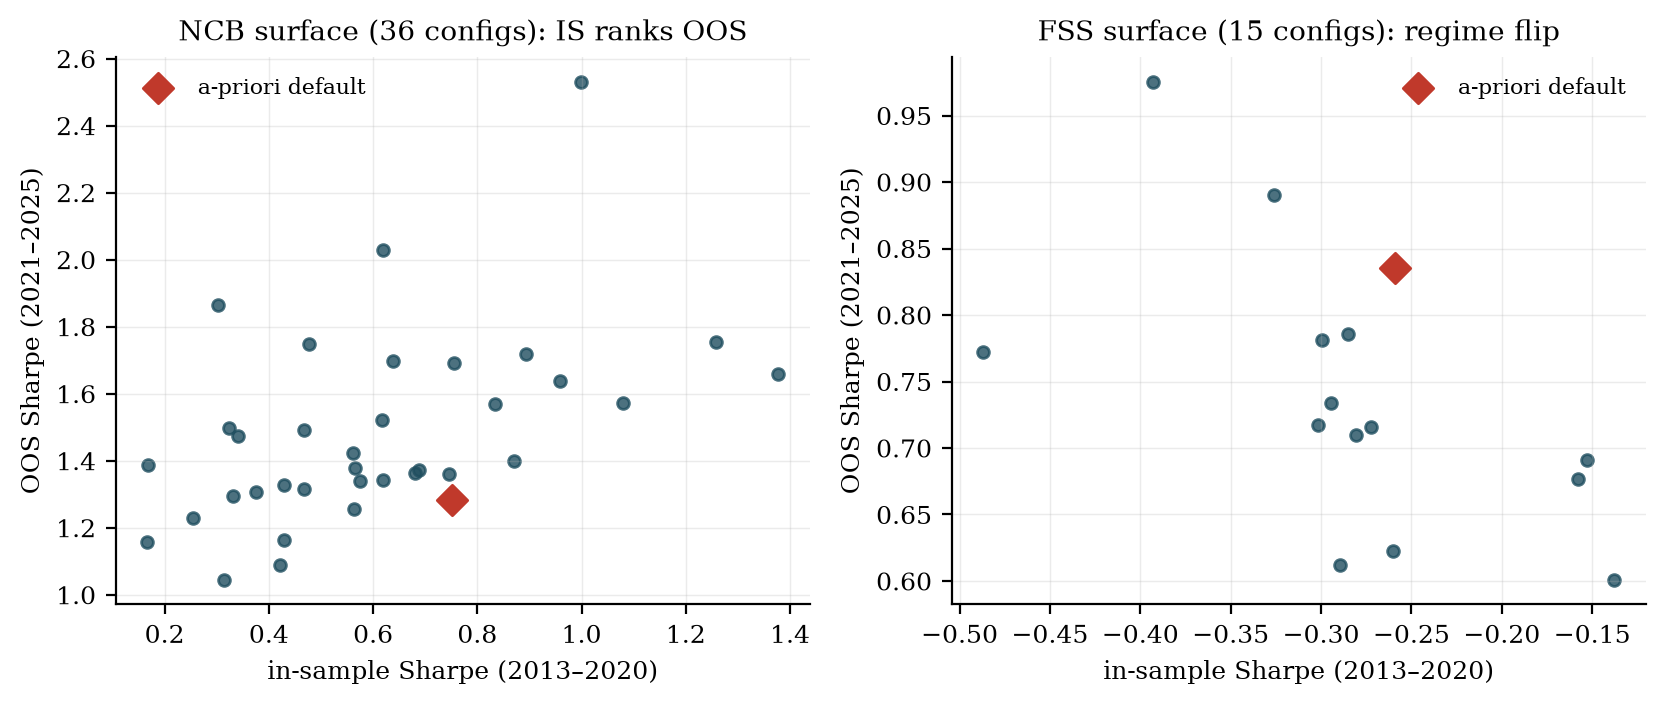
\includegraphics[width=.92\linewidth]{figs/f7_surfaces.png}
\vspace{-6pt}
\caption{Hyperparameter governance in one picture: in-sample vs
held-out Sharpe per configuration. Left, NCB: the whole surface is
positive and in-sample ranks out-of-sample ($+0.53$) --- selection
is meaningful and the a-priori default (diamond) is conservative.
Right, FSS: the grid moves as one block across a regime flip
($-0.81$) --- selection is refused and the regime is reported.}
\end{figure}

\textbf{Replications, stated as such.} CHS breadth: replicated.
Gompers--Metrick IO level and Chincarini dio/pso: dead after size,
as the modern record says. Days-of-ADV: raw VW point replicated
($+1.46\%$/mo), dies residualized --- the published effect is a
size/liquidity exposure. Agarwal confidential holdings: does not
replicate on 2013--25 ($t=-0.86$). Miori--Cucuringu imbalance
reversal: oracle form replicates; bias-adjusted (point-in-time,
churn-controlled) the premium is a fraction --- who-knew-what-when
accounting is most of the published edge. Coval--Stafford: mechanism
replicates ($t\approx+10$); expected-flow \emph{forecasting} does
not transfer to 13F-implied flows. Risk monitors that survived:
short-squeeze spikes revert ($-1.21\%$/5d after, $t=-2.6$: the
anti-panic rule is hold), and an aggregate deleveraging index
conditions risk (corr $+0.14$ with future vol, zero with returns;
gross throttle improves combo Sharpe 0.49$\to$0.55) --- state as
conditioner, never signal.

\begin{table}[h]
\centering\scriptsize
\caption{Signal catalogue, top and bottom (17 signals, headline
version fixed ex-ante by the placebo rule; 49 quarters; full table
in the report). The conviction family leads; states cluster at or
below zero.}
\begin{tabular}{llrrrr}
\toprule
signal & version & spread/q & $t$ & Sharpe & IC \\
\midrule
NCB (new conviction) & resid & $+0.0218$ & $+3.54$ & $1.08$ & $+0.023$ \\
conviction top (level) & resid & $+0.0223$ & $+2.39$ & $0.65$ & $+0.024$ \\
breadth level & resid & $+0.0193$ & $+1.48$ & $0.36$ & $+0.027$ \\
entry rate & raw & $+0.0134$ & $+1.23$ & $0.36$ & $+0.004$ \\
$\Delta$breadth (common) & raw & $+0.0049$ & $+1.07$ & $0.27$ & $+0.008$ \\
days-of-ADV (crowding) & resid & $-0.0066$ & $-0.41$ & $-0.12$ & $+0.012$ \\
holder concentration & resid & $-0.0048$ & $-1.09$ & $-0.29$ & $-0.012$ \\
$\Delta$inst.\ ownership (2q) & raw & $-0.0083$ & $-1.89$ & $-0.46$ & $-0.009$ \\
\bottomrule
\end{tabular}
\end{table}

\textbf{Low confidence / noise vs signal.} FSS's price payoff rests
on one 20-quarter regime --- hedge, not all-weather alpha. IPCA's
edge and the sharper-NCB corner are candidates pending fresh sample.
The LO tilt ordering and the Q4 quarter-end anomaly are
noise-until-replicated. Gross research spreads are systematically
kinder than net engine results; every promoted claim above is the
net one. The single strongest evidence that the survivors are real
is procedural: the same funnel retracted its own marginal result
when the data improved.

\section{The three things we would build next}

\textbf{1. CRSP-tier prices with corporate-event unification.}
Closes the one measured open bias (survivorship truncations that cut
against both legs), captures delisting returns the FSS mechanism
partly trades, unifies trading items across ticker recycling and
CUSIP reassignment via permno, lifts value coverage
85.4$\to\sim$98\% --- and every headline is re-verified by the same
campaign machinery that already caught one artifact. Highest
inferential payoff per unit of work; everything downstream inherits
it.

\textbf{2. Probabilistic position nowcasting between filings, fed by
higher-frequency flow/performance data.} The 45-day staleness is the
binding constraint on everything tactical; the oracle-vs-adjusted
replication quantifies the prize (with true positions the imbalance
premium is a multiple of the lagged version). The new data ---
monthly N-PORT portfolios plus Morningstar-tier reported TNA,
subscriptions/redemptions, and returns --- does two jobs. It feeds
the nowcast alongside inputs already validated (drifted books, the
flow instrument, real short interest supervising our synthetic proxy
at corr 0.55, mechanical ETF rebalance rules); and it re-opens flow
\emph{prediction} honestly: forecasting failed on 13F-\emph{implied}
flow (leverage and measurement error destroy its autocorrelation)
--- the literature's predictability lives in \emph{reported} flows,
with NMF-cluster hierarchical shrinkage as the waiting estimator.
Deliverable: a probabilistic estimate of \emph{current} holdings
with honest uncertainty; gate, mechanism-first: beat the frozen-book
baseline on holdings reconstruction OOS before any return claim.

\textbf{3. Fundamentals and a risk model for residualization and
false-discovery control.} The placebo currently neutralizes size and
liquidity --- the exposures 13F counting is mechanically loaded on
--- but value/quality/profitability tilts of conviction buying
remain unmodeled. Accounting data makes the theorem test
characteristic-complete, turns crowding measurement into proper
risk-model exposures, and supports \emph{joint} false-discovery
control across the catalogue instead of per-family Bonferroni: the
difference between ``NCB is not size'' (shown) and ``NCB is not any
priced characteristic'' (the next bar).

\end{document}
